
\documentclass[12pt]{ctexart}

\usepackage[a4paper,margin=2.5cm]{geometry}
\usepackage{setspace}
\usepackage{titlesec}
\usepackage{xcolor}
\usepackage{indentfirst}
\usepackage{float}
\usepackage{graphicx}
\usepackage{tikz}
\usepackage{amsmath}
\usepackage{caption}
\usepackage{subcaption}

\usetikzlibrary{arrows.meta,positioning,calc}

\setlength{\parindent}{0em}
\setstretch{1.35}
\captionsetup{font=small}

% 标题格式
\titleformat{\section}{\bfseries\zihao{4}}{}{0em}{}
\titleformat{\subsection}{\bfseries\zihao{-4}}{}{0em}{}

% 图片标题显示为“图”
\renewcommand{\figurename}{图}
\captionsetup[figure]{font=small,labelsep=space}

% 单图：带图号、标题、标签
\newcommand{\imgsingle}[4][0.82\textwidth]{
\begin{figure}[H]
    \centering
    \includegraphics[width=#1]{#2}
    \caption{#3}
    \label{#4}
\end{figure}
}

% 两张并排，但每张图各自独立编号：图1、图2
\newcommand{\imgtwosep}[7][0.47\textwidth]{
\begin{center}
    \begin{minipage}[t]{#1}
        \centering
        \includegraphics[width=\linewidth]{#2}
        \captionof{figure}{#3}
        \label{#4}
    \end{minipage}
    \hfill
    \begin{minipage}[t]{#1}
        \centering
        \includegraphics[width=\linewidth]{#5}
        \captionof{figure}{#6}
        \label{#7}
    \end{minipage}
\end{center}
}

\begin{document}

\thispagestyle{empty}

\begin{figure}[H]
    \centering
    
\includegraphics[width=0.70\textwidth]{img/0.png}
\end{figure}

\vspace{2cm}

\noindent
\hspace{1.5em}学生姓名\textbf{：}吕乐彬
\hfill
学号\textbf{：}2023080904007
\hfill
指导教师\textbf{：}李忻洋

\vspace{2cm}

\noindent {\heiti\zihao{3} 一、实验项目名称：}信息对抗综合设计实验II——文件系统及引导区实验

\vspace{0.8cm}

\noindent {\heiti\zihao{3} 二、实验目的：}

本实验以 FAT12 软盘文件系统和软盘引导区为对象，通过创建、格式化、查看和修改软盘镜像文件，理解文件在磁盘上的组织方式，以及系统从引导区获得执行权的基本过程。实验并不只是观察文件是否存在，而是进一步分析文件名、目录项、首簇号、FAT 表和数据区之间的对应关系，从而掌握文件定位和文件恢复的底层依据。

\begin{center}
\begin{tikzpicture}[
    node distance=0.95cm,
    box/.style={
        draw,
        rounded corners,
        minimum width=3.6cm,
        minimum height=0.95cm,
        align=center
    },
    core/.style={
        draw,
        rounded corners,
        minimum width=4.8cm,
        minimum height=1.0cm,
        align=center
    },
    arrow/.style={-{Stealth[length=2.2mm]}, thick}
]
\node[box] (a) {创建并格式化\\FAT12 软盘镜像};
\node[core, below=0.9cm of a] (b) {分析文件系统元数据\\目录项、FAT 表、数据区};
\node[box, below left=1.0cm and 2.4cm of b] (c) {定位文件\\实际内容};
\node[box, below=1.0cm of b] (d) {删除文件\\并尝试恢复};
\node[box, below right=1.0cm and 2.4cm of b] (e) {理解引导区\\代码执行};

\draw[arrow] (a) -- (b);
\draw[arrow] (b) -- (c);
\draw[arrow] (b) -- (d);
\draw[arrow] (b) -- (e);

\node[align=center, below=0.45cm of d] {\small 实验主线：先建立 FAT12 镜像，再从磁盘字节层面理解文件定位、删除恢复和引导执行};
\end{tikzpicture}
\end{center}

具体来说，本实验需要达到以下目的：

\begin{enumerate}
    \item 理解 FAT12 文件系统中引导区、FAT 表、根目录区和数据区的组织关系；
    \item 掌握通过目录项和 FAT 表定位文件内容的方法；
    \item 理解文件被删除后，目录项、FAT 表和数据区分别发生的变化；
    \item 掌握在数据未被覆盖时，通过修复目录项和 FAT 表恢复文件的基本原理；
    \item 理解软盘引导区代码被 BIOS 加载并执行的过程。
\end{enumerate}

\vspace{0.8cm}

\noindent {\heiti\zihao{3} 三、实验原理：}

FAT12 文件系统可以看作是一个由若干功能区域顺序组成的磁盘结构。格式化后的软盘并不是简单地存放文件内容，而是先记录文件系统参数，再通过 FAT 表和目录项建立文件名到实际数据位置之间的映射关系。

\begin{center}
\resizebox{0.96\textwidth}{!}{
\begin{tikzpicture}[
    area/.style={
        draw,
        minimum width=9.2cm,
        minimum height=0.88cm,
        align=center
    },
    note/.style={
        draw,
        rounded corners,
        align=left,
        font=\small,
        minimum width=4.2cm,
        minimum height=0.8cm
    },
    arrow/.style={-{Stealth[length=2mm]}, thick}
]
\node[area] (boot) {引导区 DBR：第 0 扇区，保存 BPB 参数和引导代码};
\node[area, below=0cm of boot] (fat1) {FAT1：第 1--9 扇区，记录簇分配与簇链};
\node[area, below=0cm of fat1] (fat2) {FAT2：第 10--18 扇区，作为 FAT1 的备份};
\node[area, below=0cm of fat2] (root) {根目录区 DIR：第 19--32 扇区，保存卷标、文件项和目录项};
\node[area, below=0cm of root, minimum height=1.15cm] (data) {数据区 DATA：第 33 扇区开始，保存文件内容和子目录内容};

\node[note, right=0.75cm of boot] (n1) {每扇区大小：\\512 字节};
\node[note, right=0.75cm of root] (n2) {根目录区起始偏移：\\$(1+18)\times512=9728=0x2600$};
\node[note, right=0.75cm of data] (n3) {簇 2 对应\\数据区起点};

\draw[arrow] (boot.east) -- (n1.west);
\draw[arrow] (root.east) -- (n2.west);
\draw[arrow] (data.east) -- (n3.west);
\end{tikzpicture}
}
\end{center}

根目录区中的每个目录项占 32 字节。一个目录项并不直接保存文件内容，而是保存文件名、属性、首簇号和文件大小等信息。其中最关键的是首簇号，因为它指向文件在数据区中的起始位置。

\begin{center}
\resizebox{0.96\textwidth}{!}{
\begin{tikzpicture}[
    field/.style={
        draw,
        minimum height=0.88cm,
        align=center,
        font=\small
    },
    note/.style={font=\small, align=center},
    arrow/.style={-{Stealth[length=2mm]}, thick}
]
\node[field, minimum width=3.1cm] (name) {DIR\_Name\\0x00--0x0A};
\node[field, minimum width=1.6cm, right=0cm of name] (attr) {属性\\0x0B};
\node[field, minimum width=3.0cm, right=0cm of attr] (reserve) {时间日期等字段};
\node[field, minimum width=2.2cm, right=0cm of reserve] (clus) {首簇号\\0x1A};
\node[field, minimum width=2.2cm, right=0cm of clus] (size) {文件大小\\0x1C};

\node[note, below=0.5cm of name] {文件名或卷标名};
\node[note, below=0.5cm of attr] {区分文件\\目录\\卷标};
\node[note, below=0.5cm of clus] {定位数据区};
\node[note, below=0.5cm of size] {验证占用簇数};

\draw[arrow] (clus.south) -- ++(0,-0.35);
\draw[arrow] (size.south) -- ++(0,-0.35);
\end{tikzpicture}
}
\end{center}

FAT 表的作用是记录簇之间的连接关系。对于 FAT12 来说，每个 FAT 项占 12 bit，也就是 1.5 字节。文件系统根据目录项中的首簇号进入 FAT 表，再顺着 FAT 项中记录的下一簇号继续查找，直到遇到文件结束标志；在本实验示例中，通常以 $FFF$ 表示簇链结束。

\begin{center}
\begin{tikzpicture}[
    node distance=0.9cm,
    box/.style={
        draw,
        rounded corners,
        minimum width=2.2cm,
        minimum height=0.95cm,
        align=center
    },
    chain/.style={
        draw,
        circle,
        minimum size=0.9cm,
        align=center
    },
    arrow/.style={-{Stealth[length=2mm]}, thick}
]
\node[box] (dir) {目录项\\首簇号 $N$};
\node[box, right=1.2cm of dir] (fat1) {$FAT[N]=M$};
\node[box, right=1.0cm of fat1] (fat2) {$FAT[M]=K$};
\node[box, right=1.0cm of fat2] (fat3) {$FAT[K]=FFF$};

\draw[arrow] (dir) -- (fat1);
\draw[arrow] (fat1) -- (fat2);
\draw[arrow] (fat2) -- (fat3);

\node[chain, below=1.35cm of fat1] (c1) {$N$};
\node[chain, right=1.2cm of c1] (c2) {$M$};
\node[chain, right=1.2cm of c2] (c3) {$K$};

\draw[arrow] (c1) -- (c2);
\draw[arrow] (c2) -- (c3);

\node[align=center, below=0.65cm of c2] {\small 文件最终占用的簇链：$N \rightarrow M \rightarrow K$};
\end{tikzpicture}
\end{center}

在默认 FAT12 软盘中，数据区从第 33 扇区开始，并且簇 2 对应数据区的起始位置。因此，当某个文件或子目录的首簇号为 $N$ 时，它在软盘镜像文件中的偏移可按下式计算：

\[
\text{Offset}(N)=\left[33+(N-2)\right]\times512
\]

例如，当某个子目录的首簇号为 $0x0015$，即十进制 21 时：

\[
\text{Offset}(21)=\left[33+(21-2)\right]\times512
=52\times512
=0x6800
\]

文件删除与恢复的原理可以用下面的过程表示。删除文件时，DOS 通常不会立刻擦除数据区中的实际内容，而是修改目录项首字节并释放 FAT 表项；只要文件内容所在的数据区没有被新文件覆盖，就有恢复的可能。

\begin{center}
\resizebox{0.96\textwidth}{!}{
\begin{tikzpicture}[
    node distance=0.75cm,
    box/.style={
        draw,
        rounded corners,
        minimum width=3.25cm,
        minimum height=0.95cm,
        align=center
    },
    arrow/.style={-{Stealth[length=2.2mm]}, thick}
]
\node[box] (before) {删除前\\目录项正常\\FAT 簇链存在};
\node[box, right=1.0cm of before] (del) {执行 del\\目录项首字节被改写};
\node[box, right=1.0cm of del] (fat) {FAT 表项释放\\数据区内容仍可能保留};
\node[box, below=0.95cm of fat] (recover) {恢复操作\\修复目录项和 FAT 链};
\node[box, left=1.0cm of recover] (after) {DOS 重新识别\\文件恢复显示};

\draw[arrow] (before) -- (del);
\draw[arrow] (del) -- (fat);
\draw[arrow] (fat) -- (recover);
\draw[arrow] (recover) -- (after);

\node[align=center, below=0.38cm of after] {\small 恢复成立的前提：原文件占用的数据簇尚未被其他文件覆盖};
\end{tikzpicture}
}
\end{center}

引导区实验的核心在于理解系统启动时执行权的转移。当虚拟机设置为从软盘启动时，BIOS 会读取软盘第一个扇区并将其加载到内存中的固定位置，然后跳转执行其中的代码。如果将自定义引导程序写入软盘镜像的第一个扇区，就可以观察到该引导程序在系统启动前获得执行权。

\begin{center}
\resizebox{0.96\textwidth}{!}{
\begin{tikzpicture}[
    node distance=0.9cm,
    box/.style={
        draw,
        rounded corners,
        minimum width=3.0cm,
        minimum height=0.95cm,
        align=center
    },
    arrow/.style={-{Stealth[length=2.2mm]}, thick}
]
\node[box] (bios) {BIOS 自检};
\node[box, right=0.9cm of bios] (read) {读取软盘\\第 0 扇区};
\node[box, right=0.9cm of read] (load) {加载到内存\\7C00H};
\node[box, right=0.9cm of load] (exec) {跳转执行\\引导代码};

\draw[arrow] (bios) -- (read);
\draw[arrow] (read) -- (load);
\draw[arrow] (load) -- (exec);

\node[align=center, below=0.45cm of load] {\small 引导区代码在操作系统正式加载前即可获得执行机会};
\end{tikzpicture}
}
\end{center}

综上，本实验的本质是通过软盘镜像直接观察文件系统的元数据，并把“文件名如何找到文件内容”“删除文件为何可能恢复”“引导区代码为何能够执行”这三个问题联系起来理解。

\vspace{0.8cm}

\noindent {\heiti\zihao{3} 四、实验环境（设备、元器件）：}

本实验在虚拟化环境中完成，不直接修改真实硬盘。实验对象是 VMware 中连接的 FAT12 软盘镜像文件，所有格式化、修改目录项、修改 FAT 表以及写入引导程序的操作都限制在该镜像文件内部。

\begin{center}
\begin{tikzpicture}[
    node distance=0.75cm,
    layer/.style={
        draw,
        rounded corners,
        minimum width=9.5cm,
        minimum height=0.9cm,
        align=center
    },
    arrow/.style={-{Stealth[length=2mm]}, thick}
]
\node[layer] (pc) {PC 主机：运行 Windows 系统};
\node[layer, below=0.35cm of pc] (tools) {实验工具：ImHex / UltraEdit / C32ASM，NASM};
\node[layer, below=0.35cm of tools] (vm) {VMware Workstation：加载 MS-DOS 虚拟机};
\node[layer, below=0.35cm of vm] (dos) {MS-DOS：执行 format、dir、copy、md、edit、del 等命令};
\node[layer, below=0.35cm of dos] (flp) {软盘镜像 flp1.flp：FAT12 文件系统与引导区实验对象};

\draw[arrow] (pc) -- (tools);
\draw[arrow] (tools) -- (vm);
\draw[arrow] (vm) -- (dos);
\draw[arrow] (dos) -- (flp);

\node[align=center, below=0.4cm of flp] {\small 实验边界：只修改虚拟软盘镜像，不修改真实磁盘};
\end{tikzpicture}
\end{center}

其中，VMware 用于提供 DOS 运行环境和软盘连接机制；MS-DOS 用于执行文件系统操作；ImHex 等十六进制编辑器用于直接观察和修改软盘镜像中的字节内容；NASM 用于生成自定义引导程序机器码。通过这些工具的配合，可以同时从“操作系统视角”和“磁盘字节视角”观察同一个 FAT12 文件系统。

\vspace{0.8cm}

%——————————————————————————————————————————————————————————————


\noindent {\color{red}\heiti\zihao{3} 五、实验步骤：}

\vspace{0.6cm}

\noindent {\heiti\zihao{4} 任务一：生成并格式化 FAT12 软盘镜像}

本任务通过 VMware 创建软盘镜像 \texttt{flp1.flp}，并在 MS-DOS 中将其格式化为 FAT12 文件系统。随后使用 ImHex 观察格式化前后的字节变化，并通过修改卷标项验证 FAT12 根目录区的作用。

\vspace{0.3cm}

\noindent {\heiti 1. 创建空白软盘镜像}

在 VMware 中为 MS-DOS 虚拟机添加软盘设备，创建软盘镜像文件 \texttt{flp1.flp}。格式化前使用 ImHex 打开该文件，可以看到镜像内容基本全为 \texttt{00}，说明此时尚未建立引导区、FAT 表和根目录区等文件系统结构。

\imgsingle[0.80\textwidth]{img/1.png}{未格式化前的软盘镜像内容}{fig:task1-blank-floppy}

\vspace{0.3cm}

\noindent {\heiti 2. 格式化软盘并设置卷标}

在 DOS 中执行 \texttt{format a: /u} 对 A 盘进行无条件格式化，并将卷标设置为本人学号后 11 位 \texttt{23080904007}。格式化完成后执行 \texttt{dir a:}，可以看到 A 盘卷标为 \texttt{23080904007}，目录内容显示 \texttt{File not found}，说明 FAT12 文件系统已创建成功，但当前尚未写入普通文件。

\imgsingle[0.80\textwidth]{img/2.png}{DOS 中格式化软盘并查看卷标}{fig:task1-format-dir}

\vspace{0.3cm}

\noindent {\heiti 3. 观察格式化后的 FAT12 结构}

格式化后弹出软盘，使 VMware 将修改写回 \texttt{flp1.flp}。重新用 ImHex 打开该镜像，可以看到起始处出现 \texttt{EB 3C 90}、\texttt{MSDOS5.0}、\texttt{FAT12} 等内容，说明第 0 扇区已经写入 FAT12 引导记录。同时，偏移 \texttt{0x200} 处出现 \texttt{F0 FF FF}，对应 FAT1 的起始位置。

\imgsingle[0.80\textwidth]{img/3.png}{格式化后的 FAT12 引导区和 FAT 表起始位置}{fig:task1-boot-sector}

\vspace{0.3cm}

\noindent {\heiti 4. 定位根目录区卷标项}

默认 FAT12 软盘中，引导区占 1 个扇区，FAT1 和 FAT2 各占 9 个扇区，因此根目录区起始偏移为：
\[
(1+9+9)\times512=9728=\texttt{0x2600}
\]
跳转到 \texttt{0x2600} 后，可以看到卷标项字节为 \texttt{32 33 30 38 30 39 30 34 30 30 37}，对应 ASCII 字符 \texttt{23080904007}。卷标后方的属性字节为 \texttt{28}，说明该目录项为卷标项。

\imgsingle[0.80\textwidth]{img/4.png}{在根目录区 \texttt{0x2600} 处定位卷标项}{fig:task1-root-label}

\vspace{0.3cm}

\noindent {\heiti 5. 修改卷标并验证}

为验证根目录区卷标项与 DOS 显示结果的对应关系，将 \texttt{0x2600} 处首字节由 \texttt{32} 修改为 \texttt{34}，即把卷标首字符从 \texttt{2} 改为 \texttt{4}，卷标由 \texttt{23080904007} 变为 \texttt{43080904007}。

\imgsingle[0.80\textwidth]{img/5.png}{修改根目录区卷标项的首字节}{fig:task1-edit-label}

保存后重新连接软盘，在 DOS 中执行 \texttt{dir a:}，可以看到卷标显示为 \texttt{43080904007}。这说明 DOS 显示的卷标并非临时生成，而是来自 FAT12 根目录区中的卷标目录项。

\imgsingle[0.80\textwidth]{img/6.png}{DOS 中验证修改后的卷标显示结果}{fig:task1-verify-label}

%——————————————————————————————————————————————————————————————

\vspace{0.6cm}

\noindent {\heiti\zihao{4} 任务二：FAT 表及文件定位}

本任务通过 \texttt{WINA20.386} 文件分析 FAT12 的文件定位过程。基本思路是：先在根目录区找到文件目录项，读取首簇号和文件大小；再根据 FAT 表追踪簇链；最后跳转到数据区验证文件内容。

\vspace{0.3cm}

\noindent {\heiti 1. 拷贝文件到软盘}

在 DOS 中执行 \texttt{copy wina20.386 a:}，随后执行 \texttt{dir a:} 查看目录。由图\ref{fig:task2-copy-wina20}可见，文件 \texttt{WINA20.386} 已成功复制到 A 盘，大小为 \texttt{9,349 bytes}。DOS 格式化信息显示每个分配单元为 \texttt{512 bytes}，因此本实验中 \(1\text{ 簇}=1\text{ 扇区}=512\text{ bytes}\)。

\imgsingle[0.80\textwidth]{img/7.png}{将 \texttt{WINA20.386} 复制到 A 盘并查看目录}{fig:task2-copy-wina20}

\vspace{0.3cm}

\noindent {\heiti 2. 在根目录区读取文件目录项}

弹出软盘后，用 ImHex 打开 \texttt{flp1.flp}，跳转到根目录区 \texttt{0x2600}。在卷标项之后可以看到 \texttt{WINA20.386} 的目录项，其起始地址为 \texttt{0x2620}。该目录项开头字节为 \texttt{57 49 4E 41 32 30 20 20 33 38 36}，对应文件名 \texttt{WINA20  386}。

根据 FAT12 目录项结构，首簇号位于相对偏移 \texttt{0x1A}，文件大小位于相对偏移 \texttt{0x1C}。因此，首簇号字段地址为 \(\texttt{0x2620}+\texttt{0x1A}=\texttt{0x263A}\)。图中该位置两个字节为 \texttt{02 00}，按小端方式解释为 \texttt{0x0002}，即该文件首簇号为 \texttt{0x0002}。

文件大小字段地址为 \(\texttt{0x2620}+\texttt{0x1C}=\texttt{0x263C}\)。图中该位置四个字节为 \texttt{85 24 00 00}，按小端方式解释为 \texttt{0x00002485 = 9349}，与 DOS 中显示的 \texttt{9,349 bytes} 一致。

\imgsingle[0.80\textwidth]{img/8.png}{在根目录区中定位 \texttt{WINA20.386} 的目录项}{fig:task2-root-wina20}

\vspace{0.3cm}

\noindent {\heiti 3. 分析 FAT 表并追踪簇链}

FAT1 从偏移 \texttt{0x200} 开始。由于 \texttt{WINA20.386} 的首簇号为 \texttt{0x0002}，因此从 \texttt{FAT[2]} 开始追踪。图\ref{fig:task2-fat-table}中 FAT 表起始字节为：

\begin{verbatim}
F0 FF FF 03 40 00 05 60 00 07 80 00 09 A0 00 0B
C0 00 0D E0 00 0F 00 01 11 20 01 13 40 01 FF 0F
\end{verbatim}

按 FAT12 的 12 bit 项解析后，\texttt{WINA20.386} 的簇链为：
\[
2 \rightarrow 3 \rightarrow 4 \rightarrow \cdots \rightarrow 20 \rightarrow FFF
\]
因此该文件占用簇 2 到簇 20，共 19 个簇，其中 \texttt{FFF} 表示簇链结束。

\imgsingle[0.80\textwidth]{img/9.png}{在 FAT 表中追踪 \texttt{WINA20.386} 的簇链}{fig:task2-fat-table}

\vspace{0.3cm}

\noindent {\heiti 4. 使用文件大小验证簇数}

\texttt{WINA20.386} 的文件大小为 \texttt{9349 bytes}，每簇大小为 \texttt{512 bytes}，因此理论占用簇数为：
\[
\left\lceil \frac{9349}{512} \right\rceil
=
\left\lceil 18.26 \right\rceil
=
19
\]
这与 FAT 表中得到的 19 个簇一致，说明目录项中的文件大小、FAT 表中的簇链以及 DOS 显示结果相互对应。

\vspace{0.3cm}

\noindent {\heiti 5. 定位文件实际内容}

默认 FAT12 软盘中，数据区从第 33 个扇区开始，因此数据区起始偏移为：
\[
33\times512=16896=\texttt{0x4200}
\]
由于 \texttt{WINA20.386} 的首簇号为 \texttt{0x0002}，而簇 2 正好对应数据区起点，所以该文件内容起始偏移为 \texttt{0x4200}。

跳转到 \texttt{0x4200} 后，可以看到开头字节为 \texttt{4D 5A}，对应 ASCII 字符 \texttt{MZ}。这是 DOS/Windows 可执行文件常见文件头，说明通过目录项和 FAT 表定位文件内容的方法正确。

\imgsingle[0.80\textwidth]{img/10.png}{根据首簇号定位 \texttt{WINA20.386} 的数据区内容}{fig:task2-data-area}




%——————————————————————————————————————————
%——————————————————————————————————————————————————————————————

\vspace{0.6cm}

\noindent {\heiti\zihao{4} 任务三：创建子目录与文件}

本任务在 A 盘根目录下创建以学号后 11 位命名的子目录，并在该目录中创建 \texttt{LVLEBIN.TXT} 文件。随后通过根目录项、子目录目录表和数据区内容，验证 FAT12 中文件和子目录的定位过程。

\vspace{0.3cm}

\noindent {\heiti 1. 创建子目录和文本文件}

在 DOS 中进入 A 盘，先创建与卷标同名的子目录，再进入该目录并创建文本文件：

\begin{verbatim}
md 23080904007
cd 23080904007
edit lvlebin.txt
\end{verbatim}

在编辑器中输入本人学号 \texttt{2023080904007}，保存退出。由图\ref{fig:task3-edit-file}可见，\texttt{LVLEBIN.TXT} 文件中已经写入该字符串。

\imgsingle[0.80\textwidth]{img/11.png}{在 DOS 编辑器中创建 \texttt{LVLEBIN.TXT} 并写入学号}{fig:task3-edit-file}

保存后执行 \texttt{dir} 查看当前目录。由图\ref{fig:task3-dir-file}可见，当前目录下出现 \texttt{LVLEBIN.TXT}，文件大小为 \texttt{15 bytes}，说明文本文件已经成功创建。

\imgsingle[0.80\textwidth]{img/12.png}{在子目录中查看 \texttt{LVLEBIN.TXT} 文件}{fig:task3-dir-file}

\vspace{0.3cm}

\noindent {\heiti 2. 在根目录区分析目录项类型}

弹出软盘后，用 ImHex 打开 \texttt{flp1.flp}，跳转到根目录区 \texttt{0x2600}。由图\ref{fig:task3-root-dir}可见，根目录区中依次出现卷标项、普通文件项和子目录项。

其中，\texttt{0x2600} 处为卷标项 \texttt{23080904007}，属性字节为 \texttt{28}；\texttt{0x2620} 处为普通文件项 \texttt{WINA20  386}，属性字节为 \texttt{20}；\texttt{0x2640} 处为新建子目录项，属性字节为 \texttt{10}。由此可见，FAT12 通过目录项中的属性字节区分卷标、普通文件和子目录。

\imgsingle[0.80\textwidth]{img/13.png}{根目录区中卷标项、普通文件项和子目录项的属性区别}{fig:task3-root-dir}

新建子目录项起始地址为 \texttt{0x2640}。根据 FAT12 目录项结构，首簇号位于相对偏移 \texttt{0x1A}，因此首簇号字段地址为 \(\texttt{0x2640}+\texttt{0x1A}=\texttt{0x265A}\)。图中该位置两个字节为 \texttt{15 00}，按小端方式解释为 \texttt{0x0015}，即该子目录的首簇号为 \texttt{0x0015}。

\vspace{0.3cm}

\noindent {\heiti 3. 定位子目录的目录表}

默认 FAT12 软盘中，数据区从第 33 个扇区开始，簇 2 对应数据区起点。对于首簇号为 \(N\) 的目录或文件，其偏移计算公式为：

\[
\text{Offset}(N)=\left[33+(N-2)\right]\times512
\]

将子目录首簇号 \(N=0x0015=21\) 代入，可得：

\[
\text{Offset}(21)=\left[33+(21-2)\right]\times512=52\times512=\texttt{0x6800}
\]

跳转到 \texttt{0x6800} 后，可以看到该子目录自己的目录表。由图\ref{fig:task3-subdir-table}可见，\texttt{0x6800} 处为当前目录项 \texttt{.}，\texttt{0x6820} 处为上级目录项 \texttt{..}，\texttt{0x6840} 处为 \texttt{LVLEBIN  TXT} 文件项。

\imgsingle[0.80\textwidth]{img/14.png}{在 \texttt{0x6800} 处定位学号子目录的目录表}{fig:task3-subdir-table}

\vspace{0.3cm}

\noindent {\heiti 4. 定位 \texttt{LVLEBIN.TXT} 文件内容}

\texttt{LVLEBIN.TXT} 的目录项起始地址为 \texttt{0x6840}。首簇号字段地址为 \(\texttt{0x6840}+\texttt{0x1A}=\texttt{0x685A}\)，图中该位置两个字节为 \texttt{16 00}，按小端方式解释为 \texttt{0x0016}，即该文本文件首簇号为 \texttt{0x0016}。文件大小字段位于 \(\texttt{0x6840}+\texttt{0x1C}=\texttt{0x685C}\)，对应字节为 \texttt{0F 00 00 00}，即文件大小为 \texttt{15 bytes}，与 DOS 中显示结果一致。

将文件首簇号 \(N=0x0016=22\) 代入数据区偏移公式：

\[
\text{Offset}(22)=\left[33+(22-2)\right]\times512=53\times512=\texttt{0x6A00}
\]

跳转到 \texttt{0x6A00} 后，可以看到 ASCII 区中出现字符串 \texttt{2023080904007}，与在 DOS 编辑器中写入的内容一致，说明通过子目录项和文件首簇号成功定位到了文本文件的实际内容。

\imgsingle[0.80\textwidth]{img/15.png}{在 \texttt{0x6A00} 处定位 \texttt{LVLEBIN.TXT} 的文件内容}{fig:task3-file-content}


%——————————————————————————————————————————————————————————————

\vspace{0.6cm}

\noindent {\heiti\zihao{4} 任务四：删除并恢复文件}

本任务删除任务三中创建的 \texttt{LVLEBIN.TXT} 文件，观察删除后目录项和 FAT 表的变化，再通过手动修改目录项和 FAT 表恢复该文件。实验重点是验证：DOS 删除文件时并不会立即清除数据区内容，而是修改目录项状态并释放 FAT 表项。

\vspace{0.3cm}

\noindent {\heiti 1. 删除 \texttt{LVLEBIN.TXT} 文件}

在 DOS 中进入学号子目录 \texttt{23080904}，先执行 \texttt{dir} 确认 \texttt{LVLEBIN.TXT} 存在，然后执行 \texttt{del lvlebin.txt} 删除文件。删除后再次执行 \texttt{dir}，可以看到目录中只剩 \texttt{.} 和 \texttt{..} 两个目录项，\texttt{LVLEBIN.TXT} 已不再显示。

\imgsingle[0.80\textwidth]{img/16.png}{DOS 中删除 \texttt{LVLEBIN.TXT} 后的目录显示}{fig:task4-delete-dos}

\vspace{0.3cm}

\noindent {\heiti 2. 观察删除后的目录项变化}

弹出软盘后，用 ImHex 打开 \texttt{flp1.flp}，跳转到子目录目录表起始位置 \texttt{0x6800}。删除前，\texttt{LVLEBIN.TXT} 的目录项位于 \texttt{0x6840}，文件名首字节为 \texttt{4C}，对应字符 \texttt{L}。删除后，图\ref{fig:task4-deleted-entry} 中 \texttt{0x6840} 处首字节变为 \texttt{E5}，其余文件名、首簇号和文件大小字段仍然保留。

\[
\texttt{4C 56 4C 45 42 49 4E 20 54 58 54}
\quad \longrightarrow \quad
\texttt{E5 56 4C 45 42 49 4E 20 54 58 54}
\]

这说明 DOS 删除文件时，首先将目录项首字节改为删除标记 \texttt{E5}，而不是立即清空整个目录项。

\imgsingle[0.80\textwidth]{img/17.png}{删除后目录项首字节变为 \texttt{E5}}{fig:task4-deleted-entry}

\vspace{0.3cm}

\noindent {\heiti 3. 观察删除后的 FAT 表变化}

任务三中已经得到 \texttt{LVLEBIN.TXT} 的首簇号为 \texttt{0x0016}，即十进制 22。删除后跳转到 FAT 表附近的 \texttt{0x220}，可以看到相关 FAT 项发生变化。图\ref{fig:task4-fat-released} 中 \texttt{0x220} 附近为 \texttt{FF 00 00}，表示 \texttt{FAT[0x15]=FFF}，而 \texttt{FAT[0x16]=000}。

其中，\texttt{FAT[0x15]} 对应学号子目录本身，仍为结束标志；\texttt{FAT[0x16]} 对应已删除的 \texttt{LVLEBIN.TXT}，被清为 \texttt{000}，表示该簇已被释放。

\imgsingle[0.80\textwidth]{img/18.png}{删除后 \texttt{LVLEBIN.TXT} 对应 FAT 项被释放}{fig:task4-fat-released}

\vspace{0.3cm}

\noindent {\heiti 4. 手动恢复目录项}

由于 \texttt{LVLEBIN.TXT} 的数据区内容尚未被覆盖，可以通过修复目录项和 FAT 表恢复文件。首先跳转到 \texttt{0x6840}，将目录项首字节从删除标记 \texttt{E5} 改回原文件名首字母 \texttt{L} 的 ASCII 编码 \texttt{4C}。修改后，右侧 ASCII 区重新显示为 \texttt{LVLEBIN TXT}。

\[
\texttt{E5} \longrightarrow \texttt{4C}
\]

\imgsingle[0.80\textwidth]{img/19.png}{将目录项首字节由 \texttt{E5} 恢复为 \texttt{4C}}{fig:task4-restore-entry}

\vspace{0.3cm}

\noindent {\heiti 5. 手动恢复 FAT 表项}

由于 \texttt{LVLEBIN.TXT} 只有 \texttt{15 bytes}，只占用一个簇，因此需要将 \texttt{FAT[0x16]} 恢复为文件结束标志 \texttt{FFF}。在 FAT 表 \texttt{0x220} 附近，将删除后的 \texttt{FF 00 00} 修改为 \texttt{FF FF 0F}，使 \texttt{FAT[0x16]} 从 \texttt{000} 恢复为 \texttt{FFF}。

\[
\texttt{FAT[0x16]}:\ \texttt{000} \longrightarrow \texttt{FFF}
\]

\imgsingle[0.80\textwidth]{img/20.png}{将 \texttt{FAT[0x16]} 恢复为文件结束标志}{fig:task4-restore-fat}

\vspace{0.3cm}

\noindent {\heiti 6. 在 DOS 中验证恢复结果}

保存软盘镜像后，重新连接软盘并进入 \texttt{A:\textbackslash23080904} 目录。执行 \texttt{dir} 后，\texttt{LVLEBIN.TXT} 重新出现在目录中，文件大小仍为 \texttt{15 bytes}；继续执行 \texttt{type lvlebin.txt}，可以看到文件内容为 \texttt{2023080904007}。

\imgsingle[0.80\textwidth]{img/21.png}{DOS 中验证 \texttt{LVLEBIN.TXT} 恢复成功}{fig:task4-recover-verify}

由此可知，本次恢复成功的关键在于两个条件：一是目录项虽然被标记删除，但除首字节外的主要字段仍然保留；二是文件原数据簇尚未被其他文件覆盖。通过恢复目录项首字节和 FAT 表项，DOS 可以重新识别该文件并读取原始内容。








%——————————————————————————————————————————————————————————————

\vspace{0.6cm}

\noindent {\heiti\zihao{4} 任务五：自定义引导程序}

本任务使用 NASM 编写一个简单的 16 位引导程序，将其写入软盘镜像第 0 扇区，并在虚拟机中验证该引导程序是否能够在系统启动时获得执行权。BIOS 启动时会读取软盘第一个扇区并执行其中代码，因此引导区程序可以在操作系统正式加载之前运行。

\vspace{0.3cm}

\noindent {\heiti 1. 编写并编译引导程序}

首先编写汇编源文件 \texttt{boot.asm}。程序从 \texttt{0x7C00} 开始执行，利用 BIOS 中断 \texttt{int 10h} 的字符输出功能，将字符串 \texttt{2023080904007} 显示在屏幕上，最后停在循环中。程序末尾填充到 \texttt{512 bytes}，并在最后两个字节写入引导扇区结束标志 \texttt{55 AA}。

随后使用 NASM 执行编译命令 \texttt{nasm boot.asm -o boot.com}，得到大小为 \texttt{512 bytes} 的 \texttt{boot.com}，满足引导扇区大小要求。

\vspace{0.3cm}

\noindent {\heiti 2. 将引导程序写入软盘镜像第 0 扇区}

使用 ImHex 打开 \texttt{boot.com} 和任务五使用的软盘镜像，将 \texttt{boot.com} 的全部 \texttt{512 bytes} 覆盖写入软盘镜像偏移 \texttt{0x0000} 开始的位置。软盘镜像开头已经变为自定义引导程序机器码，同时右侧 ASCII 区可见字符串 \texttt{2023080904007}。

\imgsingle[0.80\textwidth]{img/22.png}{格式}{}

进一步检查可见，偏移 \texttt{0x01FE} 和 \texttt{0x01FF} 处为引导结束标志 \texttt{55 AA}；从 \texttt{0x0200} 开始仍然可以看到 FAT 表内容，说明本次操作只覆盖了第 0 扇区，未破坏后续 FAT12 文件系统区域。同时，Windows 文件夹中已经生成 \texttt{boot.asm} 和 \texttt{boot.com}，说明引导程序编译文件准备完成。

\begin{figure}[!htbp]
    \centering
    \begin{subfigure}[t]{0.48\textwidth}
        \centering
        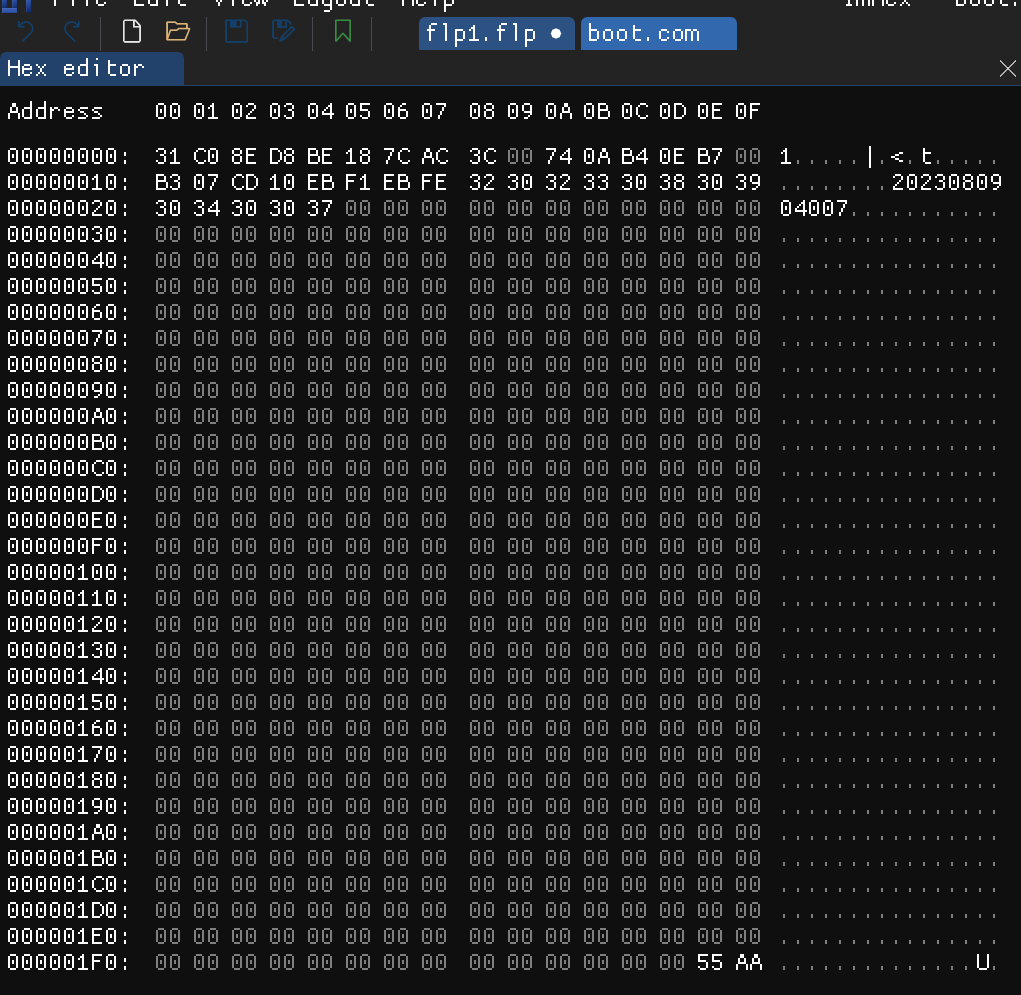
\includegraphics[width=\linewidth]{img/23.png}
        \caption{引导扇区末尾 \texttt{55 AA} 标志}
        \label{fig:task5-boot-sign}
    \end{subfigure}
    \hfill
    \begin{subfigure}[t]{0.48\textwidth}
        \centering
        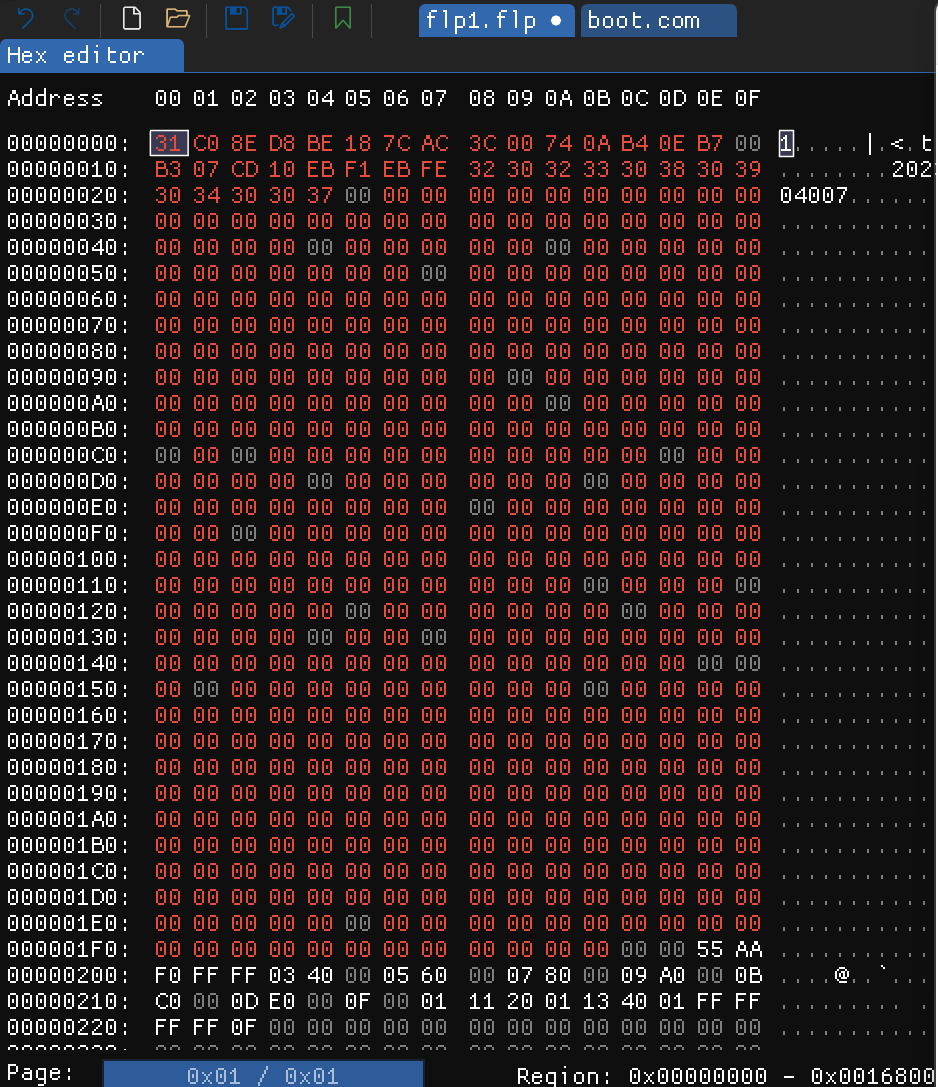
\includegraphics[width=\linewidth]{img/24.png}
        \caption{\texttt{boot.asm} 与 \texttt{boot.com} 文件}
        \label{fig:task5-boot-files}
    \end{subfigure}
    \caption{自定义引导程序写入前后的关键验证信息}
    \label{fig:task5-boot-check}
\end{figure}

\vspace{0.3cm}

\noindent {\heiti 3. 从软盘启动并验证执行结果}

将写入后的软盘镜像重新连接到 VMware 虚拟机，并设置从软盘启动。启动后，屏幕上直接显示字符串 \texttt{2023080904007}，如图\ref{fig:task5-boot-run}所示。这说明 BIOS 已成功读取软盘第一个扇区并执行其中的引导程序，系统在进入 DOS 之前就已经完成了自定义代码的执行。

\imgsingle[0.78\textwidth]{img/25.png}{虚拟机从软盘启动后显示学号}{fig:task5-boot-run}

由此可知，引导区代码确实能够在操作系统加载前获得执行权。本实验验证了 BIOS 加载软盘引导扇区的基本流程，也说明引导区是系统启动机制和安全分析中的关键位置。








\vspace{1.2cm}

\noindent {\color{red}\heiti\zihao{3} 六、实验结论：}

\vspace{0.8cm}

本实验围绕 FAT12 文件系统和软盘引导区展开，通过对软盘镜像的创建、格式化、目录项分析、FAT 表追踪、文件删除恢复以及引导程序写入与启动验证，较完整地观察了文件系统和引导机制在字节层面的实现过程。结合实验结果，可以得到以下结论：

\begin{enumerate}
    \item 格式化后的 FAT12 软盘镜像并不是简单的“空文件”，而是由引导区、FAT1、FAT2、根目录区和数据区按固定顺序组成。DOS 对软盘卷标、目录和文件的显示，本质上都依赖这些区域中的元数据。
    
    \item 根目录项保存了文件系统识别对象所需的关键信息，包括文件名、属性、首簇号和文件大小等。卷标项、普通文件项和子目录项虽然都采用 32 字节目录项结构，但可以通过属性字节分别区分，其中卷标项属性为 \texttt{28}，普通文件项属性为 \texttt{20}，子目录项属性为 \texttt{10}。
    
    \item FAT 表记录了文件占用簇之间的链接关系。通过读取目录项中的首簇号并结合 FAT 表，可以逐步追踪文件占用的全部簇，再进一步定位到数据区中的实际内容。实验中对 \texttt{WINA20.386} 和 \texttt{LVLEBIN.TXT} 的分析，都验证了目录项、FAT 表、文件大小和数据区内容之间的一致性。
    
    \item 文件删除并不等于数据立即消失。DOS 删除 \texttt{LVLEBIN.TXT} 时，只是将目录项首字节改为 \texttt{E5}，并将对应 FAT 项释放为 \texttt{000}，而数据区原始内容仍然保留。因此，只要原数据簇尚未被覆盖，就可以通过恢复目录项和 FAT 表重新找回文件。这说明文件恢复的依据并不是“猜测”，而是直接建立在文件系统结构之上的。
    
    \item 引导区代码位于软盘第 0 扇区，只要末尾包含有效引导标志 \texttt{55 AA}，BIOS 在启动时就会优先加载并执行这段代码。实验中通过自定义引导程序成功在虚拟机启动时显示学号，说明引导区确实能够在操作系统加载前获得执行权。
\end{enumerate}

综上，本实验较系统地验证了 FAT12 文件系统中“目录项负责描述对象、FAT 表负责记录簇链、数据区负责保存内容”的基本机制，同时也验证了删除恢复和引导区执行的底层原理。实验结果与指导书给出的原理是一致的，但通过亲自定位、修改和验证之后，对这些机制的理解更加具体，也更加可靠。



    \vspace{1.2cm}
\noindent {\color{red}\heiti\zihao{3} 七、总结及心得体会：}

\vspace{0.8cm}

本次实验围绕 FAT12 文件系统和软盘引导区展开。通过直接观察和修改软盘镜像，我对文件存储、删除恢复和系统启动过程有了更具体的理解。相比只看指导书中的结构说明，亲自从十六进制字节中定位目录项、FAT 表和数据区，更能看清这些机制之间的关系。

\vspace{0.35cm}

\noindent {\heiti 1. 文件不是一个孤立对象}

实验中可以看到，文件并不是只由文件名决定的。目录项保存文件名、属性、首簇号和大小，FAT 表记录簇链，数据区保存实际内容。以 \texttt{WINA20.386} 为例，目录项给出首簇号 \texttt{0x0002}，FAT 表显示其占用 19 个簇，跳转到 \texttt{0x4200} 后又能看到 \texttt{MZ} 文件头。这说明文件定位是由多个结构共同完成的。

\vspace{0.35cm}

\noindent {\heiti 2. 删除不等于擦除}

删除 \texttt{LVLEBIN.TXT} 后，DOS 中已经看不到该文件，但镜像中仍能看到目录项残留和原始数据。真正变化的是目录项首字节由 \texttt{4C} 变为 \texttt{E5}，以及 \texttt{FAT[0x16]} 由 \texttt{FFF} 变为 \texttt{000}。手动恢复这两个位置后，文件又能被 \texttt{dir} 和 \texttt{type} 正常识别。这说明普通删除只是取消文件系统索引，数据是否还能恢复取决于原数据簇是否被覆盖。

\vspace{0.35cm}

\noindent {\heiti 3. 引导区能在系统加载前执行}

在引导区实验中，将自定义引导程序写入软盘第 0 扇区，并保证末尾存在 \texttt{55 AA} 标志后，虚拟机从软盘启动时直接显示学号。这说明 BIOS 会在操作系统加载前读取并执行引导扇区代码。由此可以理解，引导区既是系统启动的关键位置，也是安全分析中需要重点关注的位置。

\vspace{0.35cm}

\noindent {\heiti 4. 实验方法上的体会}

这类底层实验不能只看现象是否“像是成功了”，而要用证据闭环验证结果。例如，修改卷标后要用 \texttt{dir a:} 验证；分析簇链后要用文件大小计算验证；恢复文件后要同时检查文件名和内容；写入引导程序后要检查 \texttt{55 AA} 并实际启动验证。通过这种“观察字节—计算偏移—修改内容—验证结果”的过程，我对文件系统和引导机制的理解比单纯阅读资料更可靠。

    \vspace{1.2cm}

\begin{flushright}
    {\heiti\zihao{3} 报告评分：}\qquad\qquad\qquad\qquad

    \vspace{1.2cm}

    {\heiti\zihao{3} 指导教师签字：}\qquad\qquad\qquad
\end{flushright}

\end{document}
